\externaldocument{../hardware_models/c-hardware_models}
\externaldocument{../astrodynamics/c-astrodynamics}
\externaldocument{../integration/c-integration}

\chapter{Phase}
\label{chap:phase}

\section{Phase base class}
\label{sec:phase_base_class}

\texttt{Phase} is the abstract base class from which all \ac{EMTG} phase types derive. The full phase class hierarchy is described in the EMTG Doxygen for the \texttt{phase} class. Every phase contains a \texttt{DepartureEvent} and an \texttt{ArrivalEvent} as described in Chapter \ref{chap:boundary-conditions}.

The base \texttt{Phase} class is also responsible for appropriately setting the stage of the spacecraft (Section \ref{sec:spacecraft}) based on user-defined values of \texttt{stage\_after\_departure}, \texttt{stage\_before\_arrival}, and \texttt{stage\_after\_arrival}.

\texttt{Phase} is responsible for calling the left and right boundaries' \texttt{calcbounds} and \texttt{process\_event} methods. \texttt{Phase} also computes the phase's initial TCM, if any, using the spacecraft's monoprop thrusters as described in Section \ref{subsec:ChemicalPropulsionSystem}.

When the phase is evaluated, \texttt{phase} calls \texttt{process\_event} on the departure and arrival events to determine the state of the spacecraft after departure and before arrival. Processing of everything that happens between the boundary points is handled by the derived phase classes as described later in this chapter.

\texttt{Phase} implements one, the time of flight ($TOF$) for the phase. The lower and upper bounds of the phase time of flight are determined based on the boundary events as described in \texttt{phase::calcbounds\_phase\_flight\_time()}.

\texttt{Phase} also implements one optional constraint. If \texttt{stage\_after\_departure} is set, then \texttt{phase} constrains the initial mass to be greater than or equal to the current stage dry mass as defined in the spacecraft definition file (Section \ref{sec:spacecraft}).

All phase classes in EMTG define the following methods:
\begin{itemize}
	\item \textbf{setup\_calcbounds()} - Sets up pointers to variable holders needed in the calcbounds process. Performs this task for not only the phase itself but also its owned departure and arrival boundary events.
	\item \textbf{calcbounds()} - Controls the calculation of bounds and sparsity pattern for the phase's decision variables and constraints by calling the below listed calcbounds methods.
	
	\item \textbf{calcbounds\_phase\_main()} - Calculates the bounds and sparsity pattern of variables and constraints defined by the derived phase class.
	
	\item \textbf{calcbounds\_virtual\_propellant\_tanks()} - Calculates the bounds and sparsity pattern of the phase's virtual propellant tank variables and constraints.
	
	\item \textbf{calcbounds\_deltav\_contribution()} - Calculates the bounds and sparsity pattern of the phase's contribution to the mission $\Delta v$. Only called when the minimum $\Delta v$ objective function is used.
	
	\item \textbf{process\_phase()} - Evaluates the phase's constraints and contribution to the objective function by calling the below listed process methods.

	\item \textbf{process\_phase\_main()} - Evaluates the phase transcription. This is always overriden by the derived class.
	
	\item \textbf{process\_phase\_left\_boundary()} - Calls the phase's departure event's process method and populates any data fields associated with the left-hand side of the phase. Handles the post-departure TCM if applicable. Handled by the base class.
	
	\item \textbf{process\_phase\_flight\_time()} - Computes the bounds on the phase time of flight. Usually handled by the base class but can be overriden for special phase types. Generally these phase types would still call the base class but then also define additional time-related variables.
	
	\item \textbf{process\_phase\_right\_boundary()} - Calls the phase's arrival event's process method and populates any data fields associated with the right-hand side of the phase. Handled by the base class.
	
	\item \textbf{process\_virtual\_propellant\_tanks()} - Computes the virtual propellant constraints, \textit{i.e.} requires that the actual propellant consumed match the virtual propellant.
	
	\item \textbf{process\_deltav\_contribution()} - Computes the phase's contribution to the total mission $\Delta v$.

	\item \textbf{output()} - Writes lines to the .emtg summary file.
	\item \textbf{output\_ephemeris()} - Writes lines to the .ephemeris file. This file may be configured to provide a high-resolution summary of systems parameters (mass, thrust, \ac{Isp}, \textit{etc.}) or may alternately be written out as just state and epoch and then used to make a SPICE kernel.
	\item \textbf{output\_maneuver\_and\_target\_spec()} - Writes lines to the .maneuver\_spec and .target\_spec files, which are used as an interface to flight-fidelity maneuver planning tools.
\end{itemize}

\section{TwoPointShootingPhase}
\label{sec:two_point_shooting_phase}

\texttt{TwoPointShootingPhase} is an abstract base class for all phase transcriptions that employ two point shooting. In other words, all phases where the spacecraft is propagated forward from the left-hand boundary condition and backward from the right-hand boundary condition. A set of match point constraints is employed to link the forward and backward half-phases together. The derivatives of the match point constraints with respect to the boundary variables may be computed via forward and backward \ac{HPTM}s, which in turn are constructed by chaining together all of the \ac{STM}s and \ac{MTM}s in the forward and backward half-phases.

\texttt{TwoPointShootingPhase} handles the creation of the match point constraints and the mapping of the partial derivatives of the boundary states to the match point constraints via the \ac{HPTM}s. Derivatives of the match point constraints with respect to variables internal to the phase, \textit{i.e.} control variables, are handled by the derived phase class.

\subsection{CoastPhase}
\label{subsec:CoastPhase}

\texttt{CoastPhase} is the simplest form of \texttt{TwoPointShootingPhase} in which the spacecraft travels from the left boundary to the right boundary without performing any maneuvers. The user may elect to propagate the trajectory via a Kepler propagator or via numerical integration with a higher-fidelity force model. In both cases, the propagation is done in the time domain.

If a numerical integrator is used, the user may independently control the step size on either side of the match point. The user specifies a time step size in seconds for the first (\texttt{CoastPhaseForward-\\IntegrationStepLength}) and second (\texttt{CoastPhaseBackwardIntegrationStepLength}) half-phase. The user may also choose \texttt{CoastPhaseMatchPointFraction} in $\left[0, 1\right]$, the fixed fraction of the phase flight time at which the match point occurs. The default value is 0.5, corresponding to a match point exactly halfway through the phase. A lower number moves the match point closer to the left-hand boundary and a higher number moves the match point closer to the right-hand boundary.

\texttt{CoastPhase} adds no new variables or constraints to the problem.

\subsection{SundmanCoastPhase}
\label{subsec:sundmancoastphase}

\texttt{SundmanCoastPhase} is identical to \texttt{CoastPhase} except that it uses a Sundman propagator instead of a time-domain propagator. An additional decision variable is added to represent the Sundman anomaly traversed over the course of the phase, and an epoch continuity constraint is added at the match point. \texttt{SundmanCoastPhase} is designed for high-fidelity modeling of gravity assists without requiring tight time steps.

\texttt{SundmanCoastPhase} is implemented in EMTGv9 with an integrated propagator and provides full analytical derivatives. The independent variable is a scaled Sundman anomaly that roughly corresponds to eccentric anomaly. EMTGv9 does not yet have a Keplerian Sundman propagator, and so SundmanCoastPhase will not work in Kepler mode. But, since Kepler mode is so fast anyway, you wouldn't want to do that.

\subsection{ControlLawThrustPhase}
\label{subsec:controlLawThrustPhase}

\texttt{ControlLawThrustPhase} is derived from \texttt{CoastPhase} but implements a finite burn using one of the spacecraft's propulsion systems, following a user-defined \texttt{ThrustControlLaw}. The user sets the journey's \texttt{thrust\_control\_law} to a value of the \texttt{ThrustControlLaw} enum. \texttt{ControlLawPhase} is then identical to \texttt{CoastPhase} except that it propagates with thrust instead of without. No additional control laws are added unless the journey\'s \texttt{thrust\_control\_law} requires them.

One new decision variable is added to represent the virtual oxidizer tank if the maneuver is biprop or the electric propellant tank if the maneuver uses the electric thruster. \hl{At the time of this writing (9/5/2020), the electric thruster for the current stage is assumed. This was deemed an acceptable behavior for now because \texttt{ControlLawThrustPhase} was developed to model a launch vehicle's injection burn and we don't want to count that against the spacecraft's chemical propellant tanks anyway. This will need to be user-selectable in the future.}

\subsection{MGAnDSMs}
\label{subsec:MGAnDSMs}

\ac{EMTG}'s Multiple Gravity Assist with \textit{n} Deep-Space Maneuvers (\texttt{MGAnDSMs}) transcription models the flight of a spacecraft using high-thrust chemical propulsion. The maneuvers are encoded as impulsive events, \textit{i.e.} they happen instantaneously, and the optimizer may place maneuvers in any permitted location in the phase. The user chooses the maximum number of impulses \textit{a priori}. If the specified number of impulses is more than what is needed, the optimizer will reduce the magnitude of any un-needed maneuvers to zero. \texttt{MGAnDSMs} derives from \texttt{TwoPointShootingPhase}.

The trajectory is propagated forward in time from the left-hand boundary condition and backward in time from the right-hand boundary condition. The optimizer chooses the time of flight ($TOF$) for the phase, along with necessary parameters to define the magnitude and direction of any impulsive \ac{DSM}s. The $TOF$ from the left-hand boundary to the first \ac{DSM}, as well as from each \ac{DSM} to the next \ac{DSM} or to the right-hand boundary where appropriate, is expressed as the product of a ``burn index'' $\eta_i$ with the phase $TOF$. The sum of the $\eta_i$ must equal 1.0, guaranteeing that the propagation arcs fit within the phase $TOF$. Therefore, if a phase has only one impulse, then the time from the left boundary to the \ac{DSM}, $\Delta t_1$, and the time from the DSM to the right boundary, $\Delta t_2$ will be:

\begin{align}
\Delta t_1 &= \eta_1 TOF\\
\Delta t_2 &= \eta_2 TOF
\label{eq:MGAnDSMs_time_calculations}
\end{align}

Mass is propagated across each impulse by means of the exponential form of the rocket equation as shown in Equation \ref{eq:rocket_equation}.

\begin{equation}
m_i^+ = m_i^- \exp \left(\frac{-\Delta v}{I_{sp} g_0}\right)
\label{eq:rocket_equation}
\end{equation}
%
where $m_i^-$ is the mass of the spacecraft before the maneuver, $m_i^+$ is the mass of the spacecraft after the maneuver, $\Delta v$ is the magnitude of the impulsive \ac{DSM}, $g_0$ is the acceleration due to gravity at sea level on Earth, and $I_{sp}$ is the specific impulse of the spacecraft's thruster. A constant mass leak term may be used to approximate propellant consumption due to \ac{ACS} desat maneuvers. \ac{EMTG} keeps track of fuel and oxidizer consumption separately so that they may be individually constrained.

The decision variables and constraints necessary to define an \ac{MGAnDSMs} phase are listed in Tables \ref{tab:decision_variables_MGAnDSMs} and \ref{tab:constraints_MGAnDSMs}, respectively. A diagram of the \ac{MGAnDSMs} phase architecture is shown in Figure \ref{fig:MGAnDSMs}. The subscript $_{mp}$ denotes that a given constraint is expressed at the match point.

\begin{figure}
	\centering
	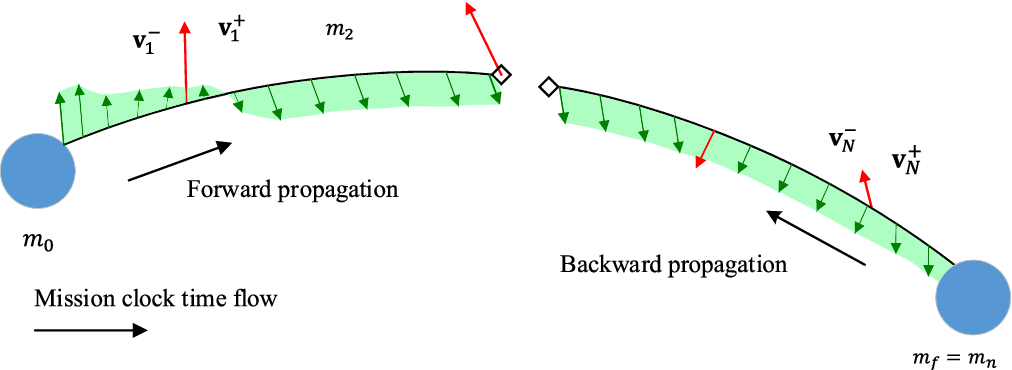
\includegraphics[width=0.8\linewidth]{MGAnDSMsphase_no_legend.png}
	\caption{\label{fig:MGAnDSMs} Diagram of the \ac{MGAnDSMs} transcription. The red arrows represent impulsive \ac{DSM}s, and the green-highlighted black arrows represent natural perturbations.}
\end{figure}

\begin{table}
	\centering
	\caption{Unique variables that define an \ac{MGAnDSMs} phase}
	\label{tab:decision_variables_MGAnDSMs}
	\begin{tabular}{ll}
		\hline\hline
		Variable & Description\\
		\hline
		$\eta_i$ &Fractions of the phase $TOF$ that define the time between \ac{DSM}s and the\\
		& boundaries, as well as between \ac{DSM}s and other \ac{DSM}s. One per \ac{DSM}\\
		& plus one for the right-hand boundary.\\
		$\Delta v_{i,x}$ & $x$ component of \ac{DSM} $i$. One per \ac{DSM}\\
		$\Delta v_{i,y}$ & $y$ component of \ac{DSM} $i$. One per \ac{DSM}\\
		$\Delta v_{i,z}$ & $z$ component of \ac{DSM} $i$. One per \ac{DSM}\\
		$m_{fuel-virtual}$ & virtual chemical fuel tank\\
		$m_{ox-virtual}$ & virtual chemical oxidizer tank\\
		\hline\hline		
	\end{tabular}
\end{table}

\begin{table}
	\centering
	\caption{Constraints that define an \ac{MGAnDSMs} phase.}
	\label{tab:constraints_MGAnDSMs}
	\begin{tabular}{ll}
		\hline\hline
		Constraint & Depends on\\
		\hline		
		$x^+_{mp} = x^-_{mp}$& $TOF$, all $\eta_i$, all $\Delta v_{i,x}$, all $\Delta v_{i,y}$, all $\Delta v_{i,z}$, boundary variables\\
		$y^+_{mp} = y^-_{mp}$& $TOF$, all $\eta_i$, all $\Delta v_{i,x}$, all $\Delta v_{i,y}$, all $\Delta v_{i,z}$, boundary variables\\
		$z^+_{mp} = z^-_{mp}$& $TOF$, all $\eta_i$, all $\Delta v_{i,x}$, all $\Delta v_{i,y}$, all $\Delta v_{i,z}$, boundary variables\\
		$\dot{x}^+_{mp} = \dot{x}^-_{mp}$& $TOF$, all $\eta_i$, all $\Delta v_{i,x}$, all $\Delta v_{i,y}$, all $\Delta v_{i,z}$, boundary variables\\
		$\dot{y}^+_{mp} = \dot{y}^-_{mp}$& $TOF$, all $\eta_i$, all $\Delta v_{i,x}$, all $\Delta v_{i,y}$, all $\Delta v_{i,z}$, boundary variables\\
		$\dot{z}^+_{mp} = \dot{z}^-_{mp}$& $TOF$, all $\eta_i$, all $\Delta v_{i,x}$, all $\Delta v_{i,y}$, all $\Delta v_{i,z}$, boundary variables\\
		$m^+_{mp} = m^-_{mp}$& $TOF$, all $\eta_i$, all $\Delta v_{i,x}$, all $\Delta v_{i,y}$, all $\Delta v_{i,z}$, boundary variables\\
		$m^+_{fuel-mp} = m^-_{fuel-mp}$& $TOF$, all $\eta_i$, all $\Delta v_{i,x}$, all $\Delta v_{i,y}$, all $\Delta v_{i,z}$, boundary variables\\
		$m^+_{ox-mp} = m^-_{ox-mp}$& $TOF$, all $\eta_i$, all $\Delta v_{i,x}$, all $\Delta v_{i,y}$, all $\Delta v_{i,z}$, boundary variables\\
		$\sum_{i=1}^{n+1} \eta_i = 1.0$ & all $\eta_i$\\
		\hline\hline		
	\end{tabular}
\end{table}

Each impulse/propagate pair in a \texttt{MGAnDSMs} phase is called a \texttt{MGAnDSMs\_subphase}. \texttt{MGAnDSMs\_subphase} is also the named of an abstract base class with two derived classes, \texttt{Forward\_MGAnDSMs\_subphase} and \texttt{Backward\_MGAnDSMs\_subphase}. These two derived classes handle the actual computation of the maneuvers and propagation of the trajectory in the forward and backward sides of the phase, respectively. The parent \texttt{MGAnDSMs} owns vectors of \texttt{Forward\_MGAnDSMs\_subphase} and \texttt{Backward\_MGAnDSMs\_subphase} objects, and is responsible for assembling the half-phase transition matrices by chaining the individual subphase state transition matrices.


\section{Probe Entry Phase}
\label{sec:ProbeEntryPhase}
\texttt{ProbeEntryPhase} is a special phase type that tracks not only the trajectory of the spacecraft, but also that of an entry probe that separates from the spacecraft and continues first to contact with the atmosphere of the Universe's central body, and then all the way to a surface target or parachute open state. \texttt{ProbeEntryPhase} derives from  \texttt{MGAnDSMs} base class. The phase's \texttt{DepartureEvent} and \texttt{ArrivalEvent}, along with all other methods and fields inherited from the base \texttt{MGAnDSMs}, correspond to the main spacecraft. \texttt{ProbeEntryPhase} contains a separate \texttt{ArrivalEvent} for the probe. The probe's \texttt{ArrivalEvent}s and second-subphase \texttt{DepartureEvent} do not interact with the rest of the problem, only with the parent \texttt{ProbeEntryPhase}. A diagram of \texttt{ProbeEntryPhase} is given in Figure \ref{fig:ProbeEntryPhase}.

\begin{figure}[ht]
	\centering
	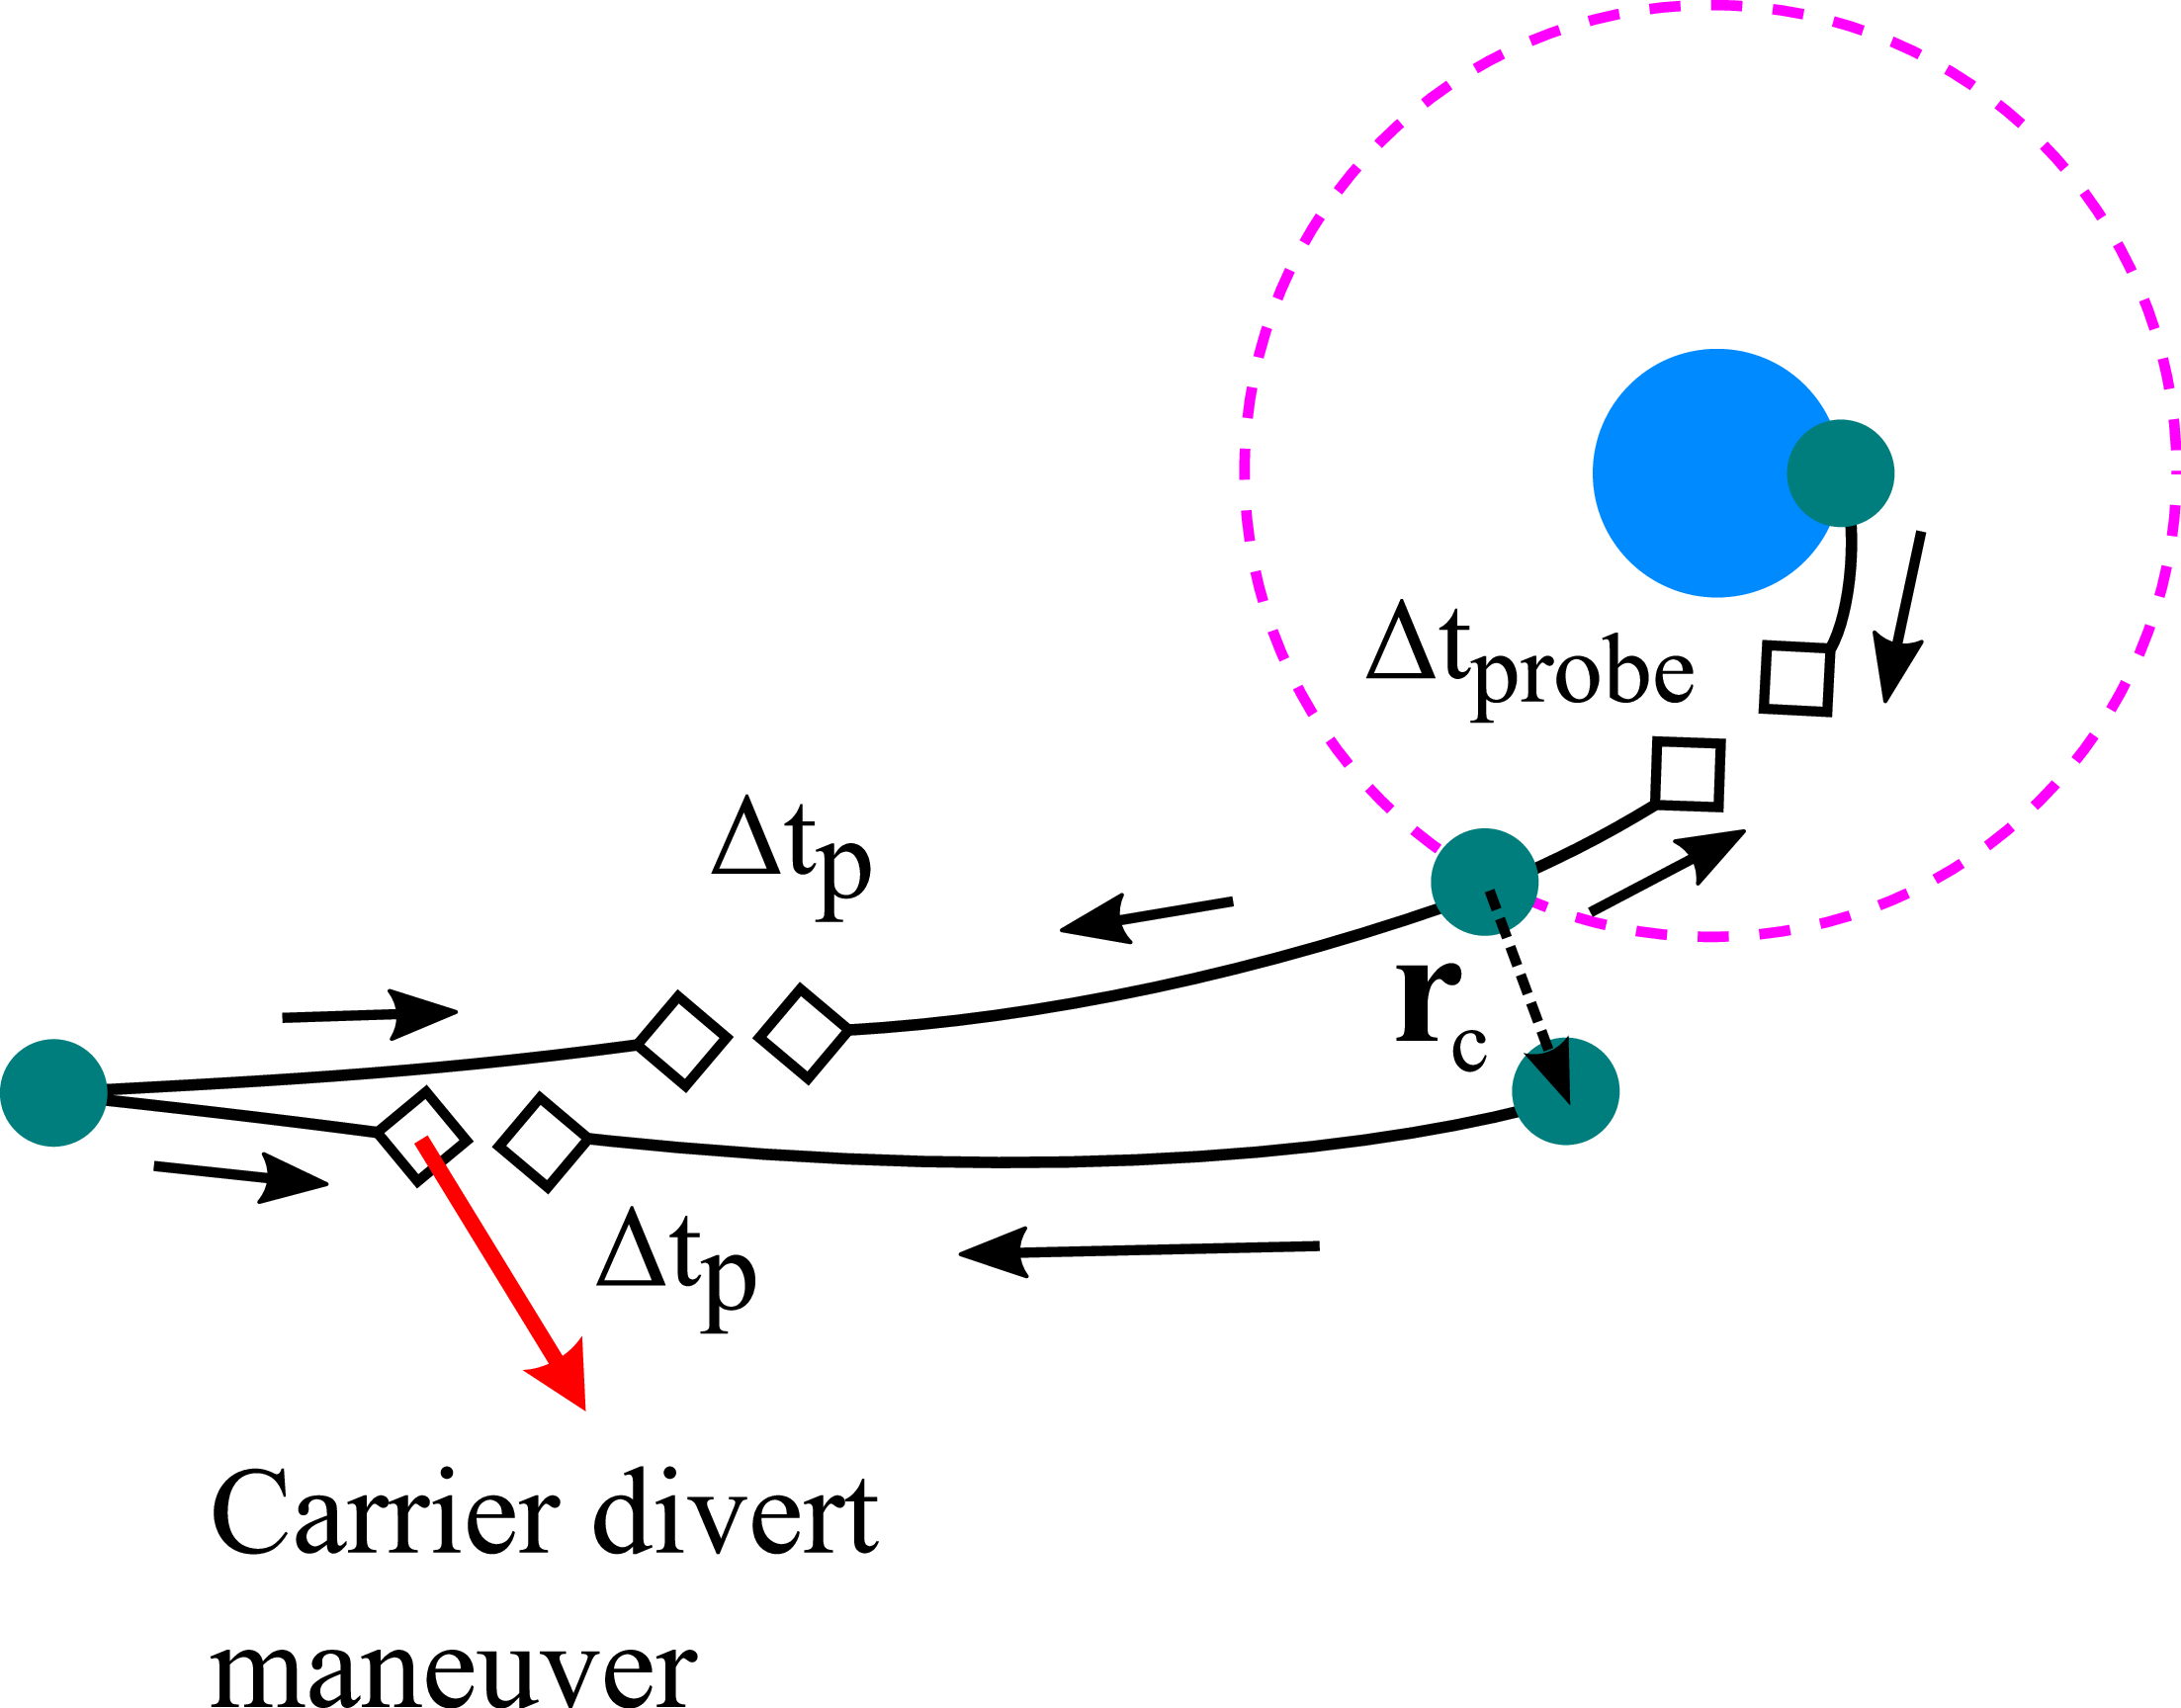
\includegraphics[width=0.7\textwidth]{ProbeEntryPhase_zoom.png}
	\caption{\label{fig:ProbeEntryPhase} The ProbeEntryPhase transcription.}
\end{figure}

The phase's \texttt{DepartureEvent} is the epoch of separation between the probe and spacecraft. Both vehicles' velocity vectors are modified by a separation impulse $I_{sep}$, which is a user-defined constant. The mass of the probe is subtracted from the mass of the spacecraft at separation. Note that in the equations below, $\mathbf{x}_{vehicle}$ is a 6-vector of inertial position and velocity.

\begin{align}
\mathbf{x}_{probe,t_s^-} &= \mathbf{x}_{s/c,t_s^-}\\
m_{s/c} &= m_{stack} - m_{probe}\\
\mathbf{x}_{probe,t_s^+} &= \mathbf{x}_{probe,t_s^-} + \left[\mathbf{0}_{3,1} \: \mathbf{I}_{sep}/m_{probe}\right]^T\\
\mathbf{x}_{s/c,t_s^+} &= \mathbf{x}_{s/c,t_s^-} + \left[\mathbf{0}_{3,1} \: \mathbf{I}_{sep}/m_{s/c}\right]^T\\
\end{align}
%
where $t_s^-$ is $\epsilon$ before separation, and $t_s^+$ is $\epsilon$ after separation. $\mathbf{I}_{sep}$ is a unit vector in the direction of the probe's velocity vector at entry. The three components of $\mathbf{I}_{sep}$ are expressed as decision variables, with a set of constraints to ensure that the direction matches the inertial velocity of the probe at the \textit{end} of the phase. The decision variables encode a velocity vector, which is then unitized to create $\mathbf{I}_{sep}$.

After separation, the probe and spacecraft are propagated separately but for the same time of flight inherited from the base \texttt{MGAnDSMs} phase. Both vehicles are propagated forward from the separation point and backward from their respective \texttt{ArrivalEvent} states. However this propagation occurs in different ways as described below.

The probe does not perform any maneuvers after separation. It is therefore propagated forward and backward to a match point whose location as a fraction of the phase time of flight is a user-defined constant. In practice the match point will be near the right-hand side so that very small time steps can be used when the probe is near the planet. This is the same approach as used in \texttt{CoastPhase} (Section \ref{subsec:CoastPhase}). The probe's right-hand boundary is currently planned as a FreePointIntercept, to which we will attach \ac{EMTG}'s standard \ac{EDL} constraints and sun zenith-angle constraints. Match-point constraints are enforced on the probe's position, velocity, and mass. The mass tracking may not be strictly necessary because the probe's mass does not evolve in time. However, we are stuck enforcing this constraint because the probe's \texttt{ArrivalEvent} is going to create a mass variable whether we like it or not and we have to tie it to something so that the \ac{NLP} solver is stable. The match point constraints are:

\begin{align}
x_{probe,mp}^+ &= x_{probe,mp}^-\\
y_{probe,mp}^+ &= x_{probe,mp}^-\\
z_{probe,mp}^+ &= x_{probe,mp}^-\\
\dot x_{probe,mp}^+ &= \dot x_{probe,mp}^-\\
\dot y_{probe,mp}^+ &= \dot y_{probe,mp}^-\\
\dot z_{probe,mp}^+ &= \dot z_{probe,mp}^-\\	
m_{probe,mp}^+ &= m_{probe,mp}^-	
\end{align}

After arriving at its first waypoint, usually constrained by the user to represent atmosphere entry, the probe proceeds through a second coast subphase that is identical to the first but with a different terminal condition. Unlike the first subphase, this second coast subphase requires its own flight time decision variable. In order to prevent the rest of \ac{EMTG} from adding it to the running count of flight time variables, the probe's second subphase flight time is stored in the list of variables as ``ProbeFlightThyme.'' Kyle Hughes would like to remind everybody that (A) thyme is delicious and (B) the name was his idea.

The spacecraft performs one maneuver, the divert, after separation. The spacecraft's match point is attached to the divert maneuver and can move in time just as in an \texttt{MGAnDSMs} phase (Section \ref{subsec:MGAnDSMs}). The forward and backward propagation times are given by:

\begin{align}
\Delta t_{s/c,forward} &= \eta_1 TOF\\
\Delta t_{s/c,backward} &= \eta_2 TOF
\end{align}
%
where $\eta_1$ and $\eta_2$ are burn index variables subject to the constraint,

\begin{align}
\eta_1 + \eta_2 = 1.0
\end{align}

The components of the divert maneuver are encoded as $\Delta v_{divert,x}$, $\Delta v_{divert,y}$, and $\Delta v_{divert,z}$, and are included in the match point constraint just as in \texttt{MGAnDSMs}.

\begin{align}
x_{s/c,mp}^+ &= x_{s/c,mp}^-\\
y_{s/c,mp}^+ &= x_{s/c,mp}^-\\
z_{s/c,mp}^+ &= x_{s/c,mp}^-\\
\dot x_{s/c,mp}^+ &= \dot x_{s/c,mp}^- + \Delta v_{divert,x}\\
\dot y_{s/c,mp}^+ &= \dot y_{s/c,mp}^- + \Delta v_{divert,y}\\
\dot z_{s/c,mp}^+ &= \dot z_{s/c,mp}^- + \Delta v_{divert,z}\\	
m_{s/c,mp}^+ &= m_{s/c,mp}^- - \Delta m_{fuel} - \Delta m_{oxidizer}
\end{align}
%
where $\Delta m_{fuel}$ and $\Delta m_{oxidizer}$ are computed as in Section \ref{subsec:MGAnDSMs}. As in Section \ref{subsec:MGAnDSMs}, a set of virtual propellant tank constraints and variables are also included.

Finally, a constraint is enforced on the distance between the probe and the spacecraft on the right-hand side of the phase. This constraint represents the need to maintain reasonably high-bandwidth communication between an entry probe and its carrier spacecraft. The constraint is enforced on the state at the end of the probe's trajectory and the state at the end of the spacecraft's trajectory:

\begin{align}
r_{probe\_to\_s/c} \leq r_{probe\_to\_s/c, max}
\end{align}

Since \texttt{ProbeEntryPhase} is derived from \texttt{MGAnDSMs} with a single maneuver, \texttt{ProbeEntryPhase} has no unique decision variables except for those defining the separation impulse and ``ProbeFlightThyme.'' All other variables that describe the spacecraft and probe are handled either by \texttt{MGAnDSMs} or by the phase \texttt{DepartureEvent} or the spacecraft or probe's respective \texttt{ArrivalEvent} and \texttt{DepartureEvent} objects, each of which behaves exactly as they do elsewhere in \ac{EMTG}.

Special care is taken to handle boundary constraints in \texttt{ProbeEntryPhase}. Any constraints on the arrival event that are specified with the standard \ac{EMTG} syntax are applied to the \textit{spacecraft\'s} \texttt{ArrivalEvent}. Any constraints suffixed by ``\texttt{\_probe\_AEI}'' are applied to the \textit{probe\'s} first subphase \texttt{ArrivalEvent}, and any constraints suffixed by ``\texttt{\_probe\_end}'' are applied to the probe\'s second subphase \texttt{ArrivalEvent}.

\subsubsection{MGAnDSMs maneuver constraints}
\label{subsubsec:MGAnDSMs_maneuver_constraints}

Each \texttt{MGAnDSMs\_subphase} contains a vector of \texttt{MGAnDSMs\_maneuver\_constraint} objects. \texttt{MGAnDSMs\_maneuver\_constraint} is an abstract base class from which a wide variety of constraints are derived. Their uses are described in the scripted constraints document. Currently we can constrain maneuver magnitude and epoch both in an absolute sense and relative to other epochs in the phase.

\texttt{MGAnDSMs\_maneuver\_constraint} objects are constructed by the \texttt{MGAnDSMs\_maneuver\_constraint\_factory}. Whenever a developer adds a new constraint, the factory must be updated.

\subsection{TwoPointShootingLowThrustPhase}
\label{subsec:TwoPointShootingLowThrustPhase}

\texttt{TwoPointShootingLowThrustPhase} is an abstract base class that is derived from \texttt{TwoPointShootingPhase}. \texttt{TwoPointShootingLowThrustPhase} is a base class for all transcriptions that model a spacecraft operating with continuous thrust (often low-thrust) propulsion for the entire phase. The user may impose forced initial and/or terminal coasts of fixed duration at the beginning and end of the phase, respectively.

Any remaining flight time not consumed by the forced coasts is available for thrusting. The thrust time is divided up into an even number of control segments, with an equal number of segments on either side of the match point. The segments are assigned equal length in the independent variable of integration. This is usually time but it is possible to construct a derived phase type that integrates over true anomaly or mean anomaly instead of time.

A control 3-vector $\mathbf{u}$ is applied at each control segment. There are 3\textit{n} control variables in a TwoPointShootingLowThrustPhase, where \textit{n} is the number of control segments. The magnitude of $\mathbf{u}$ represents the commanded duty cycle for the control segment, and is constrained to not exceed 1.0. The user may elect to force the control to have unit magnitude for all control segments, in which case the lower bound is also 1.0, or to force the control to have zero magnitude, in which case the lower and upper bounds are both 0.0. \hl{Previous versions of EMTG allowed for a fourth control variable at each step, $u_{command}$. $u_{command}$ was used to control properties of the propulsion system, such as input voltage or mass flow rate. \texttt{TwoPointShootingLowThrustPhase} does not currently support $u_{command}$ but the design allows for it to be added at a later date. The STMs and MTMs would just need an additional row and column.} The user may also elect to force the all of the control vectors in a phase to match each other, creating a fixed inertial pointing phase.

\texttt{TwoPointShootingLowThrustPhase} also implements two virtual propellant tank variables. One always represents chemical fuel, whether for main propulsion or for \ac{ACS} desats. The other represents electric propellant. These virtual tank variables may be added together to compute a linear constraint on propellant consumption across all phases and boundary events in the mission. Constraints are added to ensure that the virtual propellant variables match the actual propellant consumed in the phase. The latter is highly nonlinear and is handled with extra rows and columns in the \ac{STM} and \ac{MTM} in each derived phase class.

\hl{As of this writing, EMTG assumes that the spacecraft has single-axis articulated solar arrays. This is important because there is therefore no dependence of available power on thrust direction. Fixed arrays would have cosine losses, which are not yet modeled.}

\subsubsection{MGALT}
\label{subsubsec:MGALT}

\texttt{MGALTphase} is a low-fidelity transcription for continuous-thrust (often low-thrust) phases. It derives from \texttt{TwoPointShootingLowThrustPhase} and models the trajectory using the Sims-Flanagan transcription. The low-thrust perturbation is approximated across each control segment by a bounded impulse, where the magnitude of the impulse is equal to the maximum $\Delta v$ that could be accomplished by thrusting continuously across the thrust segment. The spacecraft is propagated between impulses by solving Kepler's equation.

The full mathematical details of the \ac{MGALT} transcription are provided in References \cite{BoundedImpulseDerivatives1} and \cite{BoundedImpulseDerivatives2}. This section discusses only the software architecture.

The calculations of available power, thrust, and mass flow rate are performed by the spacecraft model and the \texttt{BoundedImpulseManeuver} abstract base class. The mathematics of each forward or backward thrust-and-propagation step are performed by the derived \texttt{ForwardBoundedImpulseManeuver} and \texttt{BackwardBoundedImpulseManeuver} classes, respectively. The computation of derivatives is slightly different between the forward and backward versions and so two classes are necessary.

\texttt{ForwardBoundedImpulseManeuver} and \texttt{BackwardBoundedImpulseManeuver} track not only the position, velocity, and mass of the spacecraft but also the propellant state. A constant mass leak term may be used to approximate propellant consumption due to \ac{ACS} desat maneuvers. \ac{ACS} propellant is applied against the spacecraft's ``chemical fuel'' tank, whereas main propulsion is applied against the ``electric propellant'' tank.

\texttt{MGALTphase} is responsible for holding data structures, a vector of \texttt{ForwardBoundedImpulseManeuver} and \texttt{BackwardBoundedImpulseManeuver} calculation objects, and for assembling the forward and backward \ac{HPTM}s by chaining the \ac{STM}s and \ac{MTM}s as described in References \cite{BoundedImpulseDerivatives1} and \cite{BoundedImpulseDerivatives2}. \texttt{MGALTphase} also performs all file output.

The user may choose to constrain the distance between the spacecraft and any reference body at the center of each control segment. This computation is handled by the parent \texttt{MGALTphase} class. While effective, this set of constraints significantly slows the optimization process because computing the derivatives of the distance constraints with respect to the phase control variables produces a very dense sparsity pattern and requires many matrix multiplies.

\subsubsection{FBLT}
\label{subsubsec:FBLT}

\ac{FBLT} is identical to \ac{MGALT} in every way except that instead of the Sims-Flanagan transcription, \ac{FBLT} uses explicit numerical integration to propagate the equations of motion with a thrust perturbation supplied by the electric propulsion and power system models (Chapter \ref{chap:hardware_models}). Natural perturbations may also be added as described in Section \ref{sec:acceleration_model}.

\texttt{FBLTphase} derives from \texttt{TwoPointShootingLowThrustPhase} and adds no new decision variables or constraints. The user may elect to constrain the distance between the spacecraft and a reference body, as described in the scripted constraints document. As in \ac{MGALT}, the sparsity pattern of the distance constraint is a triangle and requires many \ac{STM} multiplications, and so the distance constraint adds significantly to the computation time necessary to optimize the mission.

\subsection{MGALTS}
\label{subsec:MGALTS}

\ac{MGALTS} is not yet implemented, but Donald and Jacob built a demonstrator once and will some day put it into EMTGv9 if anyone can figure out a use for it. It is just MGALT with a Sundman propagator, an additional decision variable for the Sundman anomaly traversed by the phase, and an epoch continuity constraint.

MGALTS uses a Keplerian Sundman propagator that is not yet implemented. Again, we'll build this if and when someone needs it. We did this in EMTGv8 and it worked but was not terribly useful. This subsection is a placeholder for now.

\subsection{FBLTS}
\label{subsec:FBLTS}

\ac{FBLTS} is not yet implemented, but Donald and Jacob built a demonstrator once and will some day put it into EMTGv9 if anyone can figure out a use for it. It is just FBLT with a Sundman propagator, an additional decision variable for the Sundman anomaly traversed by the phase, and an epoch continuity constraint.

FBLTS uses an integrated Sundman propagator. Again, we'll build this if and when someone needs it. We did this in EMTGv8 and it worked but was not terribly useful. This subsection is a placeholder for now.

\section{Parallel shooting phase classes}
\label{sec:parallel_shooting_phase}


\texttt{ParallelShootingPhase} is an abstract base class for phase transcriptions that model the path of a spacecraft using low-thrust propulsion via the method of direct parallel shooting \cite{enright1992}. In this technique, the phase is decomposed into a set of short shooting steps. The state vector is encoded as decision variables on the left-hand side of each short step and then propagated to the right-hand side. A set of nonlinear match point constraints are used to ensure that in a converged solution, the propagated right-hand side of the $(i-1)^{th}$ step matches the encoded left-hand side of the $i^{th}$ step. The constraints are encoded on the left-hand side of the $i^{th}$ step. The technique is called ``parallel shooting'' because all of the steps propagate in the same direction, \textit{i.e.} forward in time.

The primary role of \texttt{ParallelShootingPhase} is to hold a polymorphic vector of \texttt{ParallelShootingStep}-derived objects as described in the next paragraph. In addition, \texttt{ParallelSootingPhase} handles the forced initial and/or terminal coast if the user requests them. The terminal coast is backward propagated, unlike everything else in \texttt{ParallelShootingPhase}.

\texttt{ParallelShootingStep} is the abstract base class for a propagation step in \texttt{ParallelShootingPhase}. It handles the encoding of the left-hand side state vector and the match point constraints that connect to the right-hand side of the previous step. As of this writing, \texttt{ParallelShootingStep} can encode the state vector in \texttt{SphericalRADEC} or \texttt{SphericalAZFPA} coordinates. The match point constraints are always encoded in cartesian coordinates. \hl{Additional state and constraint representations can easily be added.} The phase type-specific derived classes of \texttt{ParallelShootingStep} are also responsible for mapping the partial derivatives of the left-hand state to the right-hand state by means of \ac{STM}s and \ac{MTM}s that are unique to that phase type. In addition to position and velocity, \texttt{ParallelShootingStep} also encodes decision variables and continuity constraints for spacecraft mass, virtual chemical fuel mass, and virtual electric propellant mass.

There are three abstract base classes that themselves derive from \texttt{ParallelShootingStep}. \texttt{ParallelShootingFirstStep} is the abstract base class for the first step in a \texttt{ParallelShootingPhase}. It is unique in that instead of retrieving right-hand propagated state information from the previous step, it pulls the state after the initial coast from the parent \texttt{ParallelShootingPhase}. \texttt{ParallelShootingLastStep} is the abstract base class for the last step in a \texttt{ParallelShootingPhase} and is unique because it has two sets of match point constraints - the usual one on the left-hand side and another set on the right-hand side to ensure that the propagated right-hand state matches the \texttt{ParallelShootingPhase}'s state prior to the terminal coast. Finally, \texttt{ParallelShootingOneStepToRuleThemAll} is an abstract base class for the special case where a \texttt{ParallelShootingPhase} has only one step and has the properties of both \texttt{ParallelShootingFirstStep} and \texttt{ParallelShootingLastStep}.

\subsection{PSFB}
\label{subsec:PSFB}

\ac{PSFB} is a transcription for modeling the path of a low-thrust spacecraft using direct parallel shooting and a high-fidelity model of both the natural and spacecraft dynamics. \ac{PSFB} consists of the \texttt{PSFBphase}, \texttt{PSFBstep}, \texttt{PSFBfirststep}, \texttt{PSFBlaststep}, and \texttt{PSFBOneStepToRuleThemAll} classes that are each derived from the corresponding base class in Section \ref{sec:parallel_shooting_phase}, as well as a \texttt{PSFBstep\_factory} that creates the various types of step.

\ac{PSFB} propagates the trajectory using explicit numerical integration as described in Chapter \ref{chap:integration} and \ac{EMTG}'s full dynamics and spacecraft model as described in Chapters \ref{chap:astrodynamics} and \ref{chap:hardware_models}. Just as in \ac{EMTG}'s other transcriptions, control is piecewise constant across a segment. The user selects to have one \textit{or more} control opportunities per segment. If more than one control opportunity is chosen then the segment is broken into equal-length control steps. Control is encoded as a 3-vector just as in \ac{MGALT} and \ac{FBLT}. \hl{There is currently no provision for a fourth control variable but it would not be too difficult to add one.} The user may elect to force the all of the control vectors in a phase to match each other, creating a fixed inertial pointing phase. The user may also elect to force the control to be either full on or full off across the phase. Figure \ref{fig:PSFB} shows a \ac{PSFB} phase.

The \ac{PSFB} derived classes are responsible only for propagation, calculation of \ac{STM}s, and output. All of the book-keeping is handled by the base classes.

\begin{figure}
	\centering
	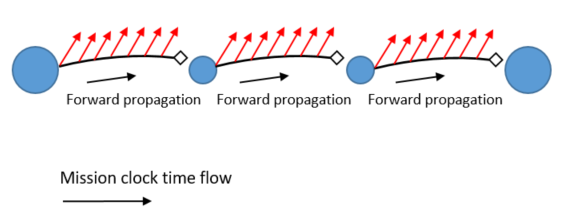
\includegraphics[width=0.8\linewidth]{PSFB.png}
	\caption{\label{fig:PSFB} Diagram of the \ac{PSFB} transcription. The red arrows represent a continuous thrust perturbation.}
\end{figure}

\FloatBarrier

\subsubsection{PSFB with high-fidelity duty cycle}
\label{subsubsec:PSFB_with_high_fidelity_duty_cycle}

\ac{PSFB}, like \ac{FBLT}, models propulsion duty cycle by multiplying the maximum duty cycle by the commanded thrust and mass flow rate. While this averaged duty cycle is sufficient for trade studies and sensitivity analysis, it may not always be acceptable as an initial guess for a flight-fidelity maneuver planning tool. \ac{EMTG} provides an alternative form of the \ac{PSFB} transcription that explicitly models the individual thrust arc and the short coast that exist in each thrust segment. The coast period is set aside for tracking, communication, other mission needs (\textit{e.g.} optical navigation), and contingencies. As with all of \ac{EMTG}'s other low-thrust transcriptions, power and propulsion characteristics are continuously evaluated as the trajectory is propagated and so thruster mode transitions can occur during a segment. Figure \ref{fig:PSFB_hifi_duty} shows three \ac{PSFB} steps with high-fidelity duty cycle modeling and thrust transitions due to a high-fidelity propulsion model.

\begin{figure}
	\centering
	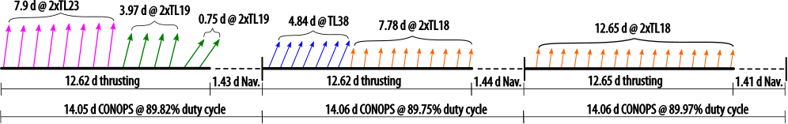
\includegraphics[width=0.8\linewidth]{PSFB_hifi_duty_cycle.png}
	\caption{\label{fig:PSFB_hifi_duty} Diagram of a three \ac{PSFB} steps with high-fidelity duty cycle modeling.}
\end{figure}

The high-fidelity duty cycle variant of \ac{PSFB} is implemented by creating yet another set of derived classes: \texttt{PSFB\_HifiDuty\_step}, \texttt{PSFB\_HifiDuty\_firststep}, \texttt{PSFB\_HifiDuty\_laststep}, and \texttt{PSFB\_HifiDuty\_OneStepToRuleTHemAll}. No new phase class is necessary because the container of \texttt{PSFBstep} objects in \texttt{PSFBphase} is polymorphic and can be populated with the high-fidelity duty cycle variants instead.

\subsection{PSBI}
\label{subsec:PSBI}

\acl{PSBI} (\acs{PSBI}) is a low-fidelity parallel-shooting transcription that combines the Sims-Flanagan model \cite{SimsFlanagan1999} with the base parallel-shooting phase classes. In \ac{PSBI}, the low-thrust acceleration is modeled as a bounded impulse in the center of each time step just as in \ac{MGALT}. Just as in \ac{PSFB}, each time-step encodes its left-hand state in the decision vector and includes a set of continuity constraints to ensure that the encoded left-hand state matches the previous step's propagated right-hand state. Figure \ref{fig:PSBI_diagram} describes the \ac{PSBI} transcription.

\begin{figure}[hb]
	\centering
	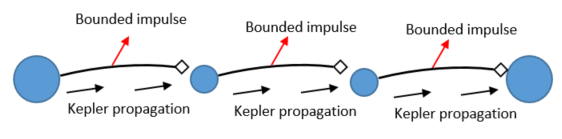
\includegraphics[width=0.8\linewidth]{PSBI.png}
	\caption{ The \ac{PSBI} transcription.}
	\label{fig:PSBI_diagram}
\end{figure}

\ac{PSBI} is composed of the \texttt{PSBIphase} container class, the \texttt{PSBIstep} base class for time steps, and the \texttt{PSBIfirststep}, \texttt{PSBIlaststep}, and \texttt{PSBIOneStepToRuleThemAll}. Each of these is derived from the corresponding abstract base class for \texttt{ParallelShootingPhase} as described in Section \ref{sec:parallel_shooting_phase}. The \ac{PSBI} step classes are constructed by \texttt{PSBIstep\_factory}.

\ac{PSBI} uses exactly the same decision variables and constraints as \ac{PSFB}, as defined in the base \texttt{ParallelShootingPhase} and child classes. Since \ac{PSBI} runs much faster than \ac{PSFB}, this enables the user to quickly converged a solution in \ac{PSBI} and then use it as an initial guess for \ac{PSFB}.

\subsection{Parallel Shooting Constraints}
\label{subsec:parallel_shooting_constraints}

The base \texttt{ParallelShootingStep} class contains vectors of \texttt{ParallelShootingStepDistanceConstraint} and \texttt{ParallelShootingStep\_maneuver\_constraint} objects. These constraints are enforced on the left-hand side of each segment. \texttt{ParallelShootingStepDistanceConstraint} is a stand-alone class that there is no need to inherit from as far as we can think of. Its use is described in the scripted constraints document.

\texttt{ParallelShootingStep\_maneuver\_constraint} is an abstract base class that is designed so that a developer may easily write derived classes to constraint maneuver magnitude, direction, etc. As of this writing (12/27/2019), there is only one such derived constraint, the Body-Probe-Thrust (BPT) angle constraint. This constraint is described in detail in the scripted constraints document. Maneuver constraints are the primary reason to use \ac{PSFB} and \ac{PSBI} instead of \ac{FBLT} and \ac{MGALT}. Maneuver constraints are very difficult to pose in a two-point shooting transcription but very easy in a parallel shooting transcription because the state vector at the left-hand side of each segment is encoded into the decision vector and no chaining is necessary.

\texttt{ParallelShootingStep\_maneuver\_constraint} objects are constructed by the \texttt{ParallelShootingStep\_maneuver\_constraint\_factory}.

	
\endinput